\documentclass[11pt]{article}
\usepackage[preprint]{acl}

\usepackage{times}
\usepackage{latexsym}
\usepackage[T1]{fontenc}
\usepackage[utf8]{inputenc}
\usepackage{microtype}
\usepackage{inconsolata}
\usepackage{graphicx}
\usepackage{booktabs}
\usepackage{tabularx}
\usepackage{float}
\usepackage{longtable}
\usepackage{array}
\usepackage{amsmath,amssymb}
\usepackage{url}
\usepackage{enumitem}
\usepackage{listings}
\usepackage{colortbl}            % for \rowcolor
\definecolor{pale}{gray}{0.88}   % highlight colour for the key rows
\newcommand{\method}[1]{\texttt{\detokenize{#1}}}  % lets underscores work in method names

\lstset{
  basicstyle=\ttfamily\small,
  breaklines=true,           %lines that are too long
  columns=fullflexible,      
}



\newcolumntype{Y}{>{\raggedright\arraybackslash}X}

\newcommand{\projecttitle}{Reliable Multimodal Evaluation with Cascaded VLM Judges}
\newcommand{\course}{CS 613: Natural Language Processing}
\newcommand{\semester}{Sem-I, 2026--27}
\newcommand{\repo}{\href{https://github.com/ShardulJunagade/cascaded-selective-evaluation/tree/end-to-end-vlm-routing}{Project repository}}
\newcommand{\todo}[1]{\textcolor{red}{\textbf{[TEAM TO COMPLETE: #1]}}}

\setlength{\titlebox}{12cm}

\title{ASSIGNMENT 2 REPORT: \projecttitle
    \thanks{\course; \semester; Indian Institute of Technology Gandhinagar. Lead TA: Naren Kumar. Repository: \repo. Submission Date: 10 Oct 2026. AI Usage Disclosure: {The latex template was generated using ChatGPT 5.6. The content is ideated and written by the team, with AI used only for grammatical corrections and polishing in some places. Existing work is duely cited, and team members are fully responsible for the written text.}}}

\author{
  Patel Ridham Vijaykumar\\
  IIT Gandhinagar\\
  Roll Number: 23110238\\
  \texttt{ridham.patel@iitgn.ac.in}
  \And
  Anurag Singh\\
  IIT Gandhinagar\\
  Roll Number: 23110035\\
  \texttt{singh.anurag@iitgn.ac.in}
  \AND
  Arjun B. Dikshit\\
  IIT Gandhinagar\\
  Roll Number: 23110040\\
  \texttt{23110040@iitgn.ac.in}
  \And
  Abhinav Khot\\
  IIT Gandhinagar\\
  Roll Number: 23110006\\
  \texttt{abhinav.khot@iitgn.ac.in}
  \AND
  Parth Dembla\\
  IIT Gandhinagar\\
  Roll Number: 23110234\\
  \texttt{parth.dembla@iitgn.ac.in}
  \And
  Shardul Junagade\\
  IIT Gandhinagar\\
  Roll Number: 23110297\\
  \texttt{shardul.junagade@iitgn.ac.in}
  \AND
  Shriniket Behera\\
  IIT Gandhinagar\\
  Roll Number: 23110306\\
  \texttt{shriniket.behera@iitgn.ac.in}
  \And
  Rathod Yuvraj Rajubhai\\
  IIT Gandhinagar\\
  Roll Number: 24110293\\
  \texttt{yuvraj.rathod@iitgn.ac.in}
}
\begin{document}

\maketitle

\begin{abstract}
% Automatic evaluation is increasingly used to compare natural-language responses, but an LLM-based judge can disagree with human preferences. The project studies selective evaluation for vision-language models (VLMs), where a judge compares two responses in the context of an image and an instruction. The supplied implementation builds a 31,635-pair image-grounded preference corpus from five public sources and evaluates four open-weight VLM judges using cached predictions. The existing comparison includes direct judging, confidence heuristics, point-estimate calibration, and stage-wise selective certification. The repository also implements an end-to-end certification strategy that evaluates the frozen cascade as a single policy. On the reported 1,000-example benchmark, the global raw-confidence policy obtains 91.08\% accuracy on answered examples at 25.20\% coverage, while the learned-router policy obtains 90.42\% accuracy at 15.43\% coverage. The learned router does not improve coverage in this experiment.

Automatic evaluation is increasingly used to compare natural-language responses, but LLM-based judges can disagree with human preferences. We study selective evaluation for vision-language models (VLMs), in which a judge compares two responses using an image and a natural-language instruction. We construct a corpus of 31,635 image-grounded preference pairs from five public sources and evaluate four open-weight VLM judges using cached predictions. We compare direct judging, confidence heuristics, point-estimate calibration, and stage-wise selective certification. We also evaluate an end-to-end certification method that treats the frozen cascade as a single policy. On the 1,000-example benchmark, the global raw-confidence policy achieves 91.08\% selective accuracy at 25.20\% coverage, while the learned-router policy achieves 90.42\% selective accuracy at 15.43\% coverage. Thus, the learned router does not improve coverage over raw-confidence routing in this experiment.
\end{abstract}

\noindent\textbf{Keywords:} Vision-language models, LLM-as-a-judge, selective evaluation, cascaded evaluation, statistical certification

% =========================================================
\section{Introduction}

\subsection{Motivation}
Automatic evaluation is becoming important as language and vision-language systems produce more outputs than can be manually judged. However, LLMs are not always reliable judges of response quality, and prior work has raised concerns about the validity and reliability of LLM-based evaluators when their decisions are treated as authoritative without calibration \citep{chehbouni2025neither}. The \emph{Trust or Escalate} framework addresses this problem in text-only settings by allowing a judge to answer when its confidence passes a calibrated threshold and otherwise escalating the example to a stronger evaluator \citep{jung2024trust}.

We extend this risk-controlled approach to multimodal judging. A VLM judge must compare candidate responses using an image and a natural-language instruction. This setting introduces potential errors related to visual grounding and modality bias. We evaluate whether selective and cascaded policies can control disagreement with human preferences while retaining useful coverage.

\subsection{Problem Type and Research Question}
For each instance, the judge receives an image, an instruction, and two candidate responses. A human-preference label is used for evaluation. The system predicts which candidate is preferred. Unlike a conventional classifier that must answer every instance, a selective judge may abstain, while a cascade may escalate an uncertain instance to another judge. The central question is whether end-to-end certification of a complete cascade can retain the required selective accuracy while answering more instances than separate stage-wise certification.

We compare existing policies and examine two end-to-end routing scores: the cached confidence of the current judge and a learned correctness score built from features of the judge outputs. Our claims are limited to the evaluated four-judge benchmark and its repeated-split evaluation.
\section{Mentor Feedback and Discussion}
\label{sec:mentor-feedback}

Discussions with the mentor shaped several design choices. For each point below we state what was suggested, what we implemented, and why.

\paragraph{VLMs first, omni models later.} Both vision-language model (VLM) and Omni models handle inputs such as audio and video but they have different architectures, and the strongest models are proprietary. The mentor advised building and validating the pipeline with open-weight VLMs first, and offered help with API credits if proprietary models are tried later. We therefore use only open-weight VLM judges, so that the method is validated before any proprietary cost is incurred.

\paragraph{Dataset mixing.} The Assignment~1 corpus came from a single source, and a single source can carry its own biases. The mentor discussed the dataset pipeline in several weekly meetings. We replaced it with a mixture of five public preference datasets in one common format, with response positions randomized, so that no single source's biases determine the result.

\paragraph{Cascade length.} A cascade is an ordered chain of judges in which each judge answers if confident and otherwise passes the example to the next. The mentor suggested using a longer chain than the three judges of the original text-only method, to check whether performance improves as stages are added. We therefore compared three- and four-judge cascades and adopted four judges from four model families (Table~\ref{tab:models}).

\paragraph{Hypothesis testing.} The mentor asked us to evaluate our central hypothesis on a GPU cluster before 4 October. The hypothesis is that using the whole cascade as one policy lets it answer more examples than using each stage separately, with the same  target accuracy. We ran both approaches on the same judge outputs, and Tables~\ref{tab:baseline-results} and~\ref{tab:global-results} report the comparison.

\paragraph{Cost of larger judges.} Each example needs $3\times2\times4=24$ forward passes (prompts $\times$ response orders $\times$ judges), so cost grows quickly with larger judges. The mentor suggested LoRA (training a small set of added weights) and model sharding (splitting weights across GPUs) to make larger models practical. Neither helped: LoRA changes the weights but not the 24 passes per example, and sharding on an A40 did not reduce inference time much. The mentor also recommended trying Gemma 4, an open-weight Google model. Therefore we used models with comparable sizes as Gemma 4.
% =========================================================
\section{Related Work}

\subsection{Selective Evaluation of Language Model Judges}
Jung et al. introduce \emph{Trust or Escalate: LLM Judges with Provable Guarantees for Human Agreement}, which calibrates a confidence threshold so that a judge answers only on a selected subset of examples \citep{jung2024trust}. The cascade applies this decision rule in sequence: if the current judge does not meet its acceptance criterion, the example is escalated to a stronger judge. Confidence in the original method is estimated using simulated annotators, formed by prompting the judge with different few-shot preference examples.

Let $Y$ denote the human-preference label, and let $\widehat{Y}_{\pi}$ be the decision made by a policy $\pi$ when it answers. The selective risk of the policy is
\begin{equation}
R(\pi)=\Pr(\widehat{Y}_{\pi}\ne Y\mid \pi\text{ answers}).
\label{eq:selective-risk}
\end{equation}
Selective accuracy on answered examples is $1-R(\pi)$. Coverage is the fraction of evaluation examples on which the policy answers. The target parameter $\alpha$ controls the maximum permitted selective risk, while $\delta$ denotes the allowed probability that the statistical certificate fails. These quantities describe different requirements: a policy can reach high accuracy by answering very few examples, so accuracy must be reported together with coverage.

\subsection{Vision-Language Models as Judges}
The multimodal setting requires preference examples that pair visual context with natural-language instructions and two responses. The supplied data pipeline combines VisionArena, MM-RLHF, RLHF-V, VisIT-Bench, and JudgeAnything. These sources differ in how preference labels are produced, including user votes, expert scores, human corrections, worker majorities, and battle outcomes \citep{chou2024visionarena,zhang2025mmrlhf,yu2024rlhfv,bitton2023visitbench,pu2025judgeanything}.

%  =========================================================
% \section{Problem formulation}
% % \subsection{Problem Formulation and Evaluation Targets}
% The experiment compares selective evaluation policies under a target selective accuracy of $1-\alpha=0.85$, where $\alpha=0.15$. Certificates use $\delta=0.1$, corresponding to a nominal 90\% confidence level. The core deployment quantity is the selective risk in Equation~\ref{eq:selective-risk}. Coverage is reported alongside selective accuracy because abstaining on most examples can otherwise produce an uninformative high-accuracy result.

% The reported benchmark evaluates policy behavior on repeated group-safe splits. For each repetition, calibration or certification data are separated from the final test partition. The end-to-end experiment additionally reserves a router-training partition so that the routing score and candidate threshold grid are defined without using certification labels.


\section{Problem Formulation}

Let an evaluation instance be
\[
    X=(V,Q,R_0,R_1),
\]
where $V$ is an image, $Q$ is a natural-language instruction, and
$R_0$ and $R_1$ are two candidate responses. The human-preference label
$Y\in\{0,1\}$ indicates which candidate response is preferred.

The system contains an ordered sequence of $M$ vision-language model judges,
denoted by
\[
    J_1,J_2,\ldots,J_M.
\]
For an instance $X$, judge $J_j$ produces a probability distribution
$p_j(y\mid X)$ over the two candidates. Its predicted preference is
\[
    \widehat{Y}_j
    =
    \arg\max_{y\in\{0,1\}}p_j(y\mid X),
\]
and its confidence score is denoted by $S_j(X)$.

A selective cascade policy $\pi$ processes the judges sequentially. After
observing the output of judge $J_j$, the policy may take one of three actions:

\begin{enumerate}
    \item accept $\widehat{Y}_j$ as the final prediction;
    \item escalate the instance to judge $J_{j+1}$; or
    \item abstain without returning a preference.
\end{enumerate}

Accordingly, the output of the policy is
\[
    \widehat{Y}_{\pi}(X)\in\{0,1,\bot\},
\]
where $\bot$ denotes abstention. Define the answer indicator
\[
    A_{\pi}(X)
    =
    \mathbb{1}\!\left[\widehat{Y}_{\pi}(X)\neq\bot\right].
\]

The selective risk of the policy is its probability of disagreeing with the
human preference, conditioned on returning an answer:
\begin{equation}
    R(\pi)
    =
    \Pr\!\left(
        \widehat{Y}_{\pi}(X)\neq Y
        \mid A_{\pi}(X)=1
    \right).
    \label{eq:problem-selective-risk}
\end{equation}

The corresponding selective accuracy is
\[
    \operatorname{Acc}(\pi)=1-R(\pi).
\]
The coverage of the policy is the probability that it returns an answer:
\begin{equation}
    C(\pi)
    =
    \Pr\!\left(A_{\pi}(X)=1\right).
    \label{eq:problem-coverage}
\end{equation}

Selective accuracy must be considered together with coverage. A policy could
obtain high accuracy by answering only a small number of easy instances.
Conversely, a policy that answers every instance may have an unacceptably high
error rate. The primary objective is therefore to maximize coverage subject
to an upper bound $\alpha$ on selective risk:
\begin{equation}
    \max_{\pi}\; C(\pi)
    \qquad
    \text{subject to}
    \qquad
    R(\pi)\leq\alpha.
    \label{eq:problem-objective}
\end{equation}

Because the policy is selected using a finite calibration sample
$\mathcal{C}$, the risk constraint must hold with confidence
$1-\delta$:
\begin{equation}
    \Pr_{\mathcal{C}}
    \left(
        R(\pi_{\mathcal{C}})\leq\alpha
    \right)
    \geq 1-\delta.
    \label{eq:problem-guarantee}
\end{equation}

Here, $\alpha$ specifies the maximum acceptable error among answered
instances, while $\delta$ specifies the allowed probability that the
finite-sample certificate fails.

A secondary objective is to reduce evaluation cost. Let
$L_{\pi}(X)\in\{1,\ldots,M\}$ denote the number of judges called for instance
$X$, with an instance that reaches the end of the cascade charged for all
$M$ judges. The expected evaluation cost is
\begin{equation}
    K(\pi)=\mathbb{E}[L_{\pi}(X)].
\end{equation}

The complete problem is therefore to construct a selective cascade that:

\begin{enumerate}
    \item satisfies the selective-risk constraint with confidence
          $1-\delta$;
    \item maximizes the fraction of instances answered; and
    \item avoids unnecessary calls to more expensive judge stages.
\end{enumerate}

\section{Baselines}

% \subsection{Baselines}
% Abhinav
The work we are doing i.e establishing a framework for VLM judging where we can provide a changeable human agreement guarantee ($1 -\alpha$) has not been done in this space before. Thus we establish our own baselines (some of these are extensions of baselines from Trust or Escalate \cite{DBLP:conf/iclr/JungB025} adapted to multimodal context). Some of them are - one judge directly (we evaluate for for all 4 VLM judges), directly using the confidence metric's output to compare against our threshold $1 -\alpha$ to check whether to accept the result (basically we dont calibrate the threshold here, also this method is tested only for the strongest judge i.e the biggest VLM model), cascaded evaluation where we see if the current judge outputs confidence above $1 - \alpha$ - else we escalate, point-estimate calibration (basically - we calibrate here but we dont include an UCB) and stage-wise cascaded certification (Main method proposed in Trust or Escalate paper \cite{jung2024trust}). It also includes variants that change how prompts and response orderings are combined with simulated annotator style. 

Table \ref{tab:baselines} summarizes these methods in a short manner.

\begin{table*}[t]
\centering
\small
\begin{tabularx}{\textwidth}{@{}p{0.30\textwidth} Y@{}}
\toprule
\textbf{Method} & \textbf{Description} \\
\midrule
\method{direct:<judge>} & Always use one selected judge. \\
\method{heuristic:<judge>} & Answer iff confidence is above the threshold $1-\alpha$. \\
\method{cascaded_heuristic} & Same as \texttt{heuristic:<judge>}, but if a judge does not answer, the example is escalated to the next stronger judge. \\
\method{point_estimate:<judge>} & Calibrate the threshold without an UCB. \\
\method{cascaded_selective} & The same setup proposed in \cite{jung2024trust}. \\
\midrule
\method{setup:vanilla_single:<judge>} & Use a single simulated annotator. \\
\method{setup:position_swap:<judge>} & Use a single simulated annotator on both response orderings, average the two probabilities, and pick the higher one. \\
\method{setup:swap_consistency:<judge>} & Swap the order of the two responses in the simulated annotator prompt and accept the judgement only if both orders give the same answer. \\
\method{setup:prompt_order_vote:<judge>} & Take a majority vote over all simulated annotators and both response orderings. \\
\method{setup:consistency_escalation} & Same as swap\_consistency but escalate if one judge fails to answer.\\
\bottomrule
\end{tabularx}
\caption{Description of our baselines.}
\label{tab:baselines}
\end{table*}
% abhinav

% \section{Novel Contributions}
% \subsection{End-to-End Certification}
% The stage-wise method certifies a separate conditional risk for each judge stage. With $M$ judges, it allocates a failure probability of $\delta/M$ to each stage and combines the claims using a union bound. This is sufficient for an overall guarantee, but it can be conservative: later judges receive only instances rejected by earlier stages, so their calibration subsets can be small. In addition, each stage must satisfy the same risk target even though the final policy's overall risk depends on the coverage-weighted combination of stage decisions.

% The end-to-end method instead certifies the risk of the complete frozen policy:
% \begin{equation}
% R(\pi_{\tau}) = \Pr(\widehat{Y}_{\pi_{\tau}}\ne Y\mid \pi_{\tau}\text{ answers})\leq\alpha.
% \label{eq:global-risk}
% \end{equation}
% Because the target claim concerns one frozen policy, the method uses the full $\delta=0.1$ for its end-to-end certificate rather than dividing it across four stage-specific claims. Threshold candidates are determined on the router-training partition; the certification labels do not train the router or construct the threshold grid. A fixed-sequence procedure examines frozen candidates from strict to permissive, and the untouched test partition is used to report test accuracy and coverage.

% Each repeated split uses three disjoint, group-safe partitions: approximately 200 examples for router training, 300 for certification, and 500 for final testing. The original baseline comparison instead uses approximately 300 calibration examples and 700 test examples. Comparisons with the original table are therefore repeated-split aggregate comparisons, not paired test-set comparisons.

% \subsection{Routing Policies}
% \paragraph{Global raw-confidence policy.}
% The \texttt{global\_raw\_confidence} policy uses the cached confidence of the current judge as its routing score. It tests whether end-to-end certification can improve the coverage of the deployed cascade without learning a separate routing model.

% \paragraph{Global learned-router policy.}
% The \texttt{global\_learned\_router} policy uses a stage-specific logistic correctness score. The documented feature set includes cached confidence, margin, entropy, simulated-annotator vote support, probability dispersion, response-order consistency, response-order probability shift, agreement among visited model families, and earlier-stage confidence summaries. The router is trained from cached judgments, and its output is then used to select a candidate routing threshold. The source notes identify the small router-training sample as a possible reason for the learned router's weaker coverage; this explanation should be treated as a hypothesis rather than a proven cause.


\section{Novel Contributions}

\subsection{End-to-End Certification}

The stage-wise method certifies the conditional risk of each judge separately. For a cascade of $M$ judges, it assigns a failure probability of $\delta/M$ to each stage and combines the resulting guarantees using a union bound. Although this provides a guarantee for the complete cascade, it can be conservative. Later judges are calibrated only on examples rejected by the earlier stages and may therefore receive small calibration subsets. Moreover, every stage must independently satisfy the same risk target, even though the final risk is determined by the combined decisions of all stages.

We instead certify the selective risk of the complete frozen routing policy:
\begin{equation}
R(\pi_{\tau})
=
\Pr\!\left(
\widehat{Y}_{\pi_{\tau}}\ne Y
\mid
\pi_{\tau}\text{ answers}
\right)
\leq \alpha,
\label{eq:global-risk}
\end{equation}
where $\tau$ is the routing threshold. Since the certificate concerns one end-to-end policy, it uses the full failure probability $\delta=0.1$ rather than dividing it among the four judge stages.

To prevent the certification data from influencing policy construction, each repetition uses separate router-training and certification partitions. The router-training partition is used to train the routing model, where applicable, and to construct the candidate threshold grid. These candidates are then fixed before certification. The certification partition is used only to evaluate the risk bound for each candidate threshold. A fixed-sequence procedure examines the candidates from strict to permissive and returns the most permissive threshold that passes before the first failure. The test partition remains untouched until final evaluation.

Each repetition therefore uses three disjoint, group-safe partitions: approximately 200 examples for router training, 300 for certification, and 500 for testing. In comparison, the original baseline experiment uses approximately 300 calibration examples and 700 test examples. Results from the two experiments are consequently compared as aggregates over repeated splits rather than as paired results on identical test sets.

\subsection{Routing Policies}

\paragraph{Global raw-confidence policy.}
The \texttt{global\_raw\_confidence} policy uses the cached confidence produced by each VLM as its routing score. At each stage, the policy accepts the current judge's prediction if its confidence is at least $\tau$; otherwise, it continues to the next judge. It abstains if no judge reaches the threshold. This policy isolates the effect of end-to-end certification without introducing a learned routing model.

\paragraph{Global learned-router policy.}
The \texttt{global\_learned\_router} policy replaces raw VLM confidence with a stage-specific estimate of prediction correctness. For each stage, a logistic regression model is trained using cached confidence, probability margin, entropy, simulated-annotator vote support, probability dispersion, response-order consistency, response-order probability shift, agreement among the model families already visited, and summaries of earlier-stage confidence. The resulting correctness estimate is used as the routing score and is compared with the same type of globally certified threshold.

The learned router produced lower coverage than raw confidence in the reported experiment. One possible explanation is that approximately 200 router-training examples are insufficient for reliably fitting the multi-feature correctness models. The current comparison is consistent with this explanation but does not establish it as the cause.


\section{Datasets}
% Assume Everything is AI

The evaluation requires pairwise preference instances with a human reference label, more specifically an image, an instruction, two candidate responses, and a human judgement of which response is better. No single public dataset provides such instances with varied label provenance, so the corpus combines five public sources. We evolve the final corpus from the previous assignment by using additional data from quality datasets, addressing bias and filtering requirements, and projecting them onto a fixed format for processing. This section describes how each source is converted into a common format, which records are removed and why, which biases are measured, and how the data are partitioned.

\subsection{Data Sources and Label Construction}
Every source is first converted into a common record containing an image, an instruction, two responses, a preference label, the origin of that label, and metadata. The conversion is source-specific because the five sources express human preference in different ways, and only two of them provide a pairwise label directly. Table~\ref{tab:dataset-sources} summarises the sources, and the construction rules are given below.

\begin{table*}[t]
\centering
\small
\begin{tabularx}{\textwidth}{l l r r Y}
\toprule
\textbf{Source} & \textbf{Raw units} & \textbf{Converted} & \textbf{Labelled} & \textbf{Label type} \\
\midrule
VisionArena & 29,849 battles & 25,712 & 15,964 & User preference vote \\
MM-RLHF & 16,342 prompts & 8,785 & 8,650 & Pair derived from expert scores \\
RLHF-V & 5,733 rows & 5,732 & 5,716 & Human correction \\
VisIT-Bench & 5,011 judgements & 1,009 & 999 & Worker majority \\
JudgeAnything & 1,500 queries & 307 & 306 & Aggregated battle outcome \\
\midrule
\textbf{Total} & & \textbf{41,545} & \textbf{31,635} & \\
\bottomrule
\end{tabularx}
\caption{Data sources. \emph{Converted} counts the pairs produced by source-specific conversion, and \emph{Labelled} counts the pairs that remain after the shared cleaning stages and the removal of ties.}
\label{tab:dataset-sources}
\end{table*}

\textbf{VisionArena.} A user uploads an image, asks a question, and votes between the responses of two anonymous models. The judge prompt accepts a single instruction, so only single-turn battles are retained, which excludes 4,136 multi-turn battles. A vote for one model becomes the preference label, and the two tie options offered to users (``tie'' and ``both bad'') mark the record as a tie. VisionArena is the only source in which an annotator identifier refers to the same person across records.
\citep{chou2024visionarena}

\textbf{MM-RLHF.} This source contains no pairwise labels. Each prompt has several model responses, and experts score each response for faithfulness, helpfulness, and ethical considerations. We take the mean of the three scores as the quality of a response and treat a pair of responses as eligible when their mean scores differ by at least a threshold $\tau = 1.0$. The higher-scored response is the preferred one. The threshold prevents nearly equal responses from being presented as clear preferences, and it also determines how difficult the resulting comparisons are: in a sample of 2,000 prompts, 71\% have an eligible pair at $\tau = 1.0$, compared with 90\% at $\tau = 0.5$ and 33\% at $\tau = 1.5$. One eligible pair is sampled uniformly at random per prompt. Selecting the pair with the largest gap would systematically choose the easiest comparison, and retaining all pairs would introduce several correlated instances per prompt. Video prompts (2,855) and the safety subset (984) are outside the scope of the task, and 3,718 prompts have no eligible pair.
\citep{zhang2025mmrlhf}

\textbf{RLHF-V.} Each row contains a model response and a version of that response in which a human annotator has corrected hallucinated content. The corrected response is the preferred one.
\citep{yu2024rlhfv}

\textbf{VisIT-Bench.} The source provides 5,011 individual worker judgements. Judgements that refer to the same image, instruction, and response pair are grouped, giving 1,010 comparisons with approximately five judgements each. The label is the majority choice, the fraction of workers who agree with the majority is recorded as the agreement level, and an even split is treated as a tie.
\citep{bitton2023visitbench}

\textbf{JudgeAnything.} This benchmark covers fifteen task types, of which only image-to-text compares two text responses to an image. The remaining tasks produce media outputs or take video or audio as input. Of the 100 image-to-text queries, the 77 with a single image are retained, each with four model-versus-model outcomes. The label is the recorded winner, which is an aggregate over annotators and not an individual judgement.
\citep{pu2025judgeanything}

Images are handled identically for all sources. Each image is stored once, under a hash of its decoded pixels, at its original resolution. We additionally compute a perceptual hash, a compact fingerprint designed to remain unchanged under re-encoding and minor pixel-level differences. Two records are regarded as showing the same image when their perceptual hashes are identical. This definition is used in duplicate removal and in the construction of the splits.

\subsection{Processing and Filtering}
For the remainder of this section, a pair denotes one converted record: two candidate responses to the same image and instruction, together with the human label that states which response is preferred. In four sources the two responses are the outputs of two different VLMs, and in RLHF-V they are a VLM output and its human correction.

After conversion, all pairs pass through the same three stages in a fixed order, so that differences between sources in the final corpus are not caused by differences in cleaning. Table~\ref{tab:dataset-funnel} reports the number of pairs after each stage.

The first stage removes pairs in which the two responses give a judge nothing to compare. A pair is removed when its two responses are identical after lowercasing and collapsing whitespace (62 pairs), or when both responses begin with a refusal phrase (18 pairs).

The second stage removes duplicate pairs. Two pairs are duplicates when they share the same image, the same normalised instruction, and the same two responses irrespective of order, and 134 such pairs are removed. Pairs that share only the image and the instruction are retained, because several sources compare the outputs of different VLMs on one prompt and these are distinct comparisons. The dependence between such pairs is handled at the splitting stage.

The third stage separates tied pairs from labelled pairs. Agreement with a human preference is not defined when the annotator expresses no preference, so the 9,696 tied pairs are placed in a separate set and are not used in the evaluation. All but nine of them originate from VisionArena, where they amount to 38\% of the pairs that pass duplicate removal. The labelled VisionArena pairs therefore represent the comparisons on which a user expressed a preference, not all comparisons users made.

\begin{table}[t]
\centering
\small
\setlength{\tabcolsep}{4pt}
\begin{tabularx}{\linewidth}{Y r r}
\toprule
\textbf{Pipeline stage} & \textbf{Remaining} & \textbf{Removed} \\
\midrule
Source-specific conversion & 41,545 & 11,789 \\
Hygiene filtering & 41,465 & 80 \\
Duplicate removal & 41,331 & 134 \\
Tie routing & 31,635 & 9,696 \\
\midrule
Few-shot set & 3,164 & \\
Development set & 3,163 & \\
Evaluation pool & 25,308 & \\
\bottomrule
\end{tabularx}
\caption{Pairs remaining after each pipeline stage. The first row counts the multi-turn, video, safety, multi-image, and ineligible-pair exclusions described in the text. The 9,696 pairs removed by tie routing are retained as a separate set, leaving 31,635 labelled pairs, which are divided into the three partitions in the lower block.}
\label{tab:dataset-funnel}
\end{table}

\subsection{Bias Analysis}
A judge can agree with human labels for reasons unrelated to response quality if the labels correlate with a superficial property of the pair. We examine two such properties, the position of the preferred response and the response length, and one limitation specific to a single source.

\textbf{Position.} After conversion, the preferred response in RLHF-V and MM-RLHF always occupies the first position, since the correction or the higher-scored response is listed first. A judge that always selects the first response would then agree with every label from these sources. The pipeline therefore exchanges the two responses with probability one half, using a pseudo-random draw seeded by the record identifier, and flips the label and all per-annotator labels together with the responses. Table~\ref{tab:bias-checks} shows that the first-position rate is close to 50\% in every source after this step.

\textbf{Length.} The pipeline records the length of both responses and measures how often the longer response is the preferred one. This rate is between 63\% and 72\% in four sources and 51\% in VisIT-Bench. The imbalance is measured and not removed, because it is a property of the collected preferences. A judge that prefers longer responses would exceed chance agreement on these four sources without assessing content.

\textbf{Label provenance.} In RLHF-V, the preferred response is a human edit of the rejected response, which is a different comparison from one between two independently generated responses. Because the sources also differ in size by a factor of more than fifty, results are reported per source as well as in aggregate.

\begin{table}[t]
\centering
\small
\setlength{\tabcolsep}{4pt}
\begin{tabular}{lrrr}
\toprule
 & \multicolumn{2}{c}{\textbf{First preferred (\%)}} & \textbf{Longer} \\
\cmidrule(lr){2-3}
\textbf{Source} & \textbf{Before} & \textbf{After} & \textbf{wins (\%)} \\
\midrule
VisionArena & 49.7 & 50.1 & 63.0 \\
MM-RLHF & 100.0 & 50.4 & 72.5 \\
RLHF-V & 100.0 & 50.0 & 70.0 \\
VisIT-Bench & 48.6 & 51.7 & 51.0 \\
JudgeAnything & 54.6 & 47.7 & 69.2 \\
\bottomrule
\end{tabular}
\caption{Share of labelled pairs in which the first response is preferred, before and after position randomization, and share in which the longer response is preferred.}
\label{tab:bias-checks}
\end{table}

\subsection{Splits and Leakage Prevention}
The labelled pairs are divided into three partitions that serve different purposes. The few-shot set (10\%, 3,164 pairs) supplies the example comparisons that are shown to a judge inside its prompt. The development set (10\%, 3,163 pairs) is reserved for choosing hyperparameters. The evaluation pool (80\%, 25,308 pairs) is the only partition on which judges are scored. At evaluation time the pool is divided once more into a calibration set, on which the confidence thresholds of the judges are fitted, and a test set, on which agreement and coverage are measured.

These partitions must not share related pairs. If two pairs with the same image or the same prompt fall on different sides of a boundary, a judge is tested on material that it has effectively seen in its prompt or during calibration. Such pairs occur both within a source and across sources. We therefore assign groups of related pairs to partitions, and not individual pairs.

Two pairs are linked when they share the same image and instruction, or when their images have the same perceptual hash. A leakage group is a connected component under this relation, so that any two pairs joined by a chain of links belong to the same group. The 31,635 labelled pairs form 26,207 groups, and the largest contains 59 pairs (0.2\% of the corpus). Each group is assigned in full to one of the three partitions, and the pipeline verifies after assignment that no group and no image appears in two partitions.

The calibration and test sets are not fixed in advance. Each evaluation run draws them at random from the evaluation pool, again keeping every leakage group on one side, and the draw is repeated many times. A single split would show one outcome of the calibration procedure, whereas repeated draws show how often the procedure meets its target.

The results in this report are computed on a smaller benchmark and not on the full evaluation pool, because scoring four judges on 25,308 pairs exceeds the available compute. The benchmark is built in two steps. First, at most 1,000 raw rows are sampled from each source, with JudgeAnything kept in full, and passed through the same pipeline, which yields a reduced evaluation pool of approximately 2,800 pairs. Second, 1,000 pairs are selected from this reduced pool by adding whole leakage groups while keeping the share of each source close to its share in the reduced pool. The selection is deterministic. Because the same cap applies to every source, the smaller sources are represented more strongly in the benchmark than in the full corpus of Table~\ref{tab:dataset-sources}.

Each judge scores every benchmark pair six times. The pair is presented under three different prompts, each containing one few-shot example, and under both orders of the two responses, which gives 6,000 requests per judge. The resulting probabilities are stored. All baseline and routing policies are therefore evaluated on the same judge outputs, and a new threshold or policy can be evaluated without running the judges again.


% The dataset is subject to three remaining constraints. The first is access and storage,the raw sources occupy more than 40\,GB, and VisionArena can be downloaded only after its terms of use have been accepted. The second is compute.  Scoring a pair under three few-shot prompts, both response orders and four judges costs twenty-four forward passes, so the full evaluation pool would need an estimated 38 hours on an A100, which could not be obtained. The third is the limited availability of annotator identity. VisionArena is the only source that identifies individual annotators, and most of its voters contribute very few votes: 2,730 voters have at least two labelled pairs and 1,339 have at least three. Few-shot prompts that imitate a specific annotator can therefore be built for only a small group of voters from a single source.

The dataset has three remaining constraints. First, the raw sources require more than 40\,GB of storage, and VisionArena is accessible only after its terms of use have been accepted. Second, VLM inference is expensive. Each
example requires three simulated-annotator prompts, two response orderings, and four judges, giving 24 forward passes. Based on A40 profiling, scoring the complete 25,308-example evaluation pool was projected to require approximately 212 GPU-hours. We therefore used a 1,000-example benchmark, whose estimated cost was 5.6--8.4 GPU-hours. Third, annotator identities are available only
for VisionArena, and most voters contribute few labelled comparisons: 2,730 have at least two and 1,339 have at least three. Annotator-specific few-shot prompts can therefore be constructed for only a limited subset of one data source.



% =========================================================
\section{Experimental Plan}

\subsection{Risk Targets and Evaluation Design}

The experiments set the maximum permitted selective error to
$\alpha=0.15$, corresponding to a target selective accuracy of
$1-\alpha=0.85$. Certificates use $\delta=0.10$, giving a nominal certificate
confidence level of $1-\delta=0.90$. Selective accuracy is always reported
together with coverage so that a highly accurate policy that answers very few
examples is not treated as sufficient.

The reported experiments use a 1,000-example benchmark scored by all four VLM
judges. Model predictions, confidence values, and prompt/order-specific
signals are computed once and cached. All subsequent calibration, routing,
and evaluation experiments reuse these cached values and do not perform
additional VLM inference.

Evaluation is repeated over 1,000 random, group-safe partitions. Examples
that share a source group or a perceptually identical image are assigned to
the same partition to prevent related examples from appearing in both
calibration and testing. Only examples scored by every judge required for a
comparison are included, and their identities and human labels are checked
across the judge caches before evaluation.

The original baselines use a two-way partition containing approximately 300
calibration examples and 700 held-out test examples. Policies that require
calibration use the first subset to select their thresholds. Non-calibrated
baselines ignore the calibration subset but are evaluated on the same test
examples for a fair comparison.

The end-to-end routing experiment uses three disjoint subsets: approximately
200 examples for router training, 300 for certification, and 500 for final
testing. The router-training subset is used to fit the learned correctness
model and to construct the candidate threshold grid. The certification
subset selects a threshold without observing test labels. The held-out test
subset is used only to measure selective accuracy, coverage, computational
cost, and target success.

No VLM is fine-tuned in these experiments. The only trained component is the
lightweight logistic correctness model used by the learned router. The raw
confidence router requires no learned parameters. Repeating the partitioning
procedure measures the sensitivity of calibration and routing to the
available finite sample, although the repetitions are not independent
datasets because they reuse examples from the same benchmark pool.

\subsection{Judge Models and Architectural Differences}
The four-judge cascade is ordered from smaller to larger judges and spans four model families. The nominal parameter counts below are model identifiers, not a substitute for recording the exact model revision.

% \begin{table}[t]
% \centering
% \small
% \begin{tabularx}{\linewidth}{c Y p{0.18\linewidth} p{0.2\linewidth}}
% \toprule
% \textbf{Stage} & \textbf{Model} & \textbf{Nominal size} & \textbf{Family} \\
% \midrule
% 1 & Granite Vision 3.3 2B & 2B & Granite Vision \\
% 2 & Qwen2.5-VL-3B-Instruct & 3B & Qwen2.5-VL \\
% 3 & Phi-3.5-Vision-Instruct & 4.2B \\ Phi-3.5 Vision
% 4 & InternVL3-8B & 8B & InternVL3 \\
% \bottomrule
% \end{tabularx}
% \caption{Four-judge benchmark configuration documented in the repository notes. Confirm exact model revisions and parameter counts.}
% \label{tab:models}
% \end{table}

\begin{table}[t]
\centering
\small
\begin{tabularx}{\linewidth}{c Y p{0.18\linewidth} p{0.20\linewidth}}
\toprule
\textbf{Stage} & \textbf{Model} & \textbf{Parameters} & \textbf{Model family} \\
\midrule
1 & Granite Vision 3.3 2B       & 2B   & Granite Vision \\
2 & Qwen2.5-VL-3B-Instruct      & 3B   & Qwen2.5-VL \\
3 & Phi-3.5-Vision-Instruct     & 4.2B & Phi-3.5 Vision \\
4 & InternVL3-8B                & 8B   & InternVL3 \\
\bottomrule
\end{tabularx}
\caption{VLM judge sequence used in the four-stage cascade. The models increase in nominal parameter count and come from distinct model families.}
\label{tab:models}
\end{table}

No VLM fine-tuning is reported for this benchmark. The judges are run for inference and their outputs are cached. The learned routing policy is a separate lightweight correctness model trained from cached judge-output features. This distinction matters: the end-to-end extension changes how cached judgments are selected and certified rather than retraining the VLM judges themselves.

\subsection{Inference and Confidence Estimation}
Confidence is estimated using simulated annotators. The benchmark uses three prompt variants, one few-shot example for each prompt, and both candidate-response orderings. The swapped-order prediction is mapped back to the original candidate labels, and the repeated judgements are combined. The repository stores individual prompt/order predictions as well as aggregate judge outputs, permitting alternative prompt and order-combination baselines to be calculated without rerunning the models.

The scoring harness reads the probabilities of the two candidate labels directly from the model output rather than relying on generated text followed by exact string matching. It also obtains label token identifiers from the relevant tokenizer. Cached outputs are reused by the evaluation step; the reported policy comparisons do not load the VLMs or repeat inference.





% \subsection{Metrics}
% The report uses the following metrics:
% \begin{itemize}
%     \item \textbf{Selective accuracy:} fraction of answered test instances for which the judge agrees with the human preference.
%     \item \textbf{Macro accuracy:} accuracy averaged across dataset sources, reducing the dominance of larger sources.
%     \item \textbf{Coverage:} fraction of test instances answered by the policy.
%     \item \textbf{Mean judges called:} average number of judge stages visited per test instance.
%     \item \textbf{Nonempty splits:} fraction of repetitions in which the policy answers at least one test instance.
%     \item \textbf{Certified splits:} fraction of repetitions in which calibration finds a threshold that passes the certificate.
%     \item \textbf{Target success:} fraction of repetitions that both return answers and attain at least 85\% test accuracy. For heuristic and point-estimate methods this is an empirical metric, not a statistical certificate.
% \end{itemize}

% \subsection{Experimental Protocol and Ablations}
% All four-judge baseline policies are evaluated over 1,000 random, group-safe calibration/test splits on the same cached judge predictions. The end-to-end comparison uses the three-way split described above. Dataset identity and group membership are checked before evaluation, and only examples scored by all required judges are included in a comparison.

% \todo{Record the actual ablation runs and hyperparameter settings used by the team. Do not list a grid search, seed, or ablation unless it was executed and the corresponding result is available.}

\subsection{Metrics}

We evaluate each policy over $R=1000$ repeated data splits. Metrics are first
calculated separately on the held-out test set of each split and are then
averaged across splits. We do not pool predictions from different splits,
because the same example can occur in the test sets of multiple repetitions.

For split $r$, let $\mathcal{T}_r$ denote its test set, let
$n_r = |\mathcal{T}_r|$, and let $\mathcal{A}_r \subseteq \mathcal{T}_r$
contain the examples answered by the policy. A policy ``answers'' an example
when it accepts the prediction of one of the judges; otherwise, it abstains.
Let $m_r = |\mathcal{A}_r|$, and let
$\mathbb{1}[\widehat{y}_i=y_i]$ indicate whether the selected VLM prediction
agrees with the human preference.

\begin{itemize}
    \item \textbf{Selective accuracy.}
    For a nonempty split, selective accuracy is
    \[
        \operatorname{Acc}_r =
        \frac{
            \sum_{i\in\mathcal{A}_r}
            \mathbb{1}[\widehat{y}_i=y_i]
        }{m_r}.
    \]
    It therefore measures accuracy only among examples that the policy chooses
    to answer. Since this quantity is undefined when $m_r=0$, the reported
    selective accuracy is the arithmetic mean over nonempty splits:
    \[
        \operatorname{Acc} =
        \frac{1}{|\mathcal{R}_{+}|}
        \sum_{r\in\mathcal{R}_{+}}\operatorname{Acc}_r,
        \qquad
        \mathcal{R}_{+}=\{r:m_r>0\}.
    \]
    This is an unweighted mean of split-level accuracies, rather than one
    accuracy computed after pooling all answered examples. For a direct
    baseline that answers every test example, selective accuracy reduces to
    ordinary test accuracy.

    \item \textbf{Macro accuracy.}
    To prevent larger dataset sources from dominating the result, accuracy is
    also calculated separately for each source represented among the answered
    examples. If $\mathcal{D}_r^{+}$ is the set of sources with at least one
    answered example in split $r$, then
    \[
        \operatorname{MacroAcc}_r =
        \frac{1}{|\mathcal{D}_r^{+}|}
        \sum_{d\in\mathcal{D}_r^{+}}
        \frac{
            \sum_{i\in\mathcal{A}_r:\,d_i=d}
            \mathbb{1}[\widehat{y}_i=y_i]
        }{
            |\{i\in\mathcal{A}_r:d_i=d\}|
        }.
    \]
    Every represented source receives equal weight, irrespective of its number
    of examples. The reported macro accuracy is the mean of this value over
    the splits for which it is defined.

    \item \textbf{Coverage.}
    Coverage in split $r$ is the fraction of its test set answered by the
    policy:
    \[
        \operatorname{Cov}_r = \frac{m_r}{n_r}.
    \]
    Reported coverage is the mean over all $R=1000$ splits:
    \[
        \operatorname{Cov} =
        \frac{1}{R}\sum_{r=1}^{R}\operatorname{Cov}_r.
    \]
    Splits in which the policy answers nothing contribute zero coverage.
    Consequently, coverage captures both how many examples are answered when a
    policy is active and how often it abstains on an entire split.

    \item \textbf{Mean judges called.}
    This metric measures the inference cost of a cascade. For each test
    example, we count the number of judge stages visited before the policy
    accepts a prediction. If the system reaches the final judge and still
    abstains, it is charged for all four judge calls. The count is averaged
    over test examples within each split and then averaged across all splits.

    \item \textbf{Nonempty splits.}
    The nonempty rate measures how often a policy produces at least one test
    prediction:
    \[
        \operatorname{Nonempty} =
        \frac{1}{R}\sum_{r=1}^{R}\mathbb{1}[m_r>0].
    \]
    This metric is necessary because a high selective accuracy can otherwise
    be produced by a policy that answers very few examples or frequently
    abstains on the complete test set.

    \item \textbf{Certified splits.}
    For the end-to-end certified routers, a split is marked as certified when
    calibration returns a valid acceptance threshold whose one-sided
    finite-sample upper bound on selective error is at most
    $\alpha=0.15$. The certified rate is
    \[
        \operatorname{Certified} =
        \frac{\text{splits with a certified threshold}}{R}
    \]
    Certification uses only the calibration subset and does not inspect the
    test labels. If no threshold passes calibration, the implemented router
    abstains on the complete test split. Certified and nonempty rates can
    therefore be numerically equal for these routers, although the former
    describes calibration and the latter describes test-time behavior.

    \item \textbf{Target success.}
    The required selective-accuracy target is
    $1-\alpha=0.85$. A repetition is counted as successful only when the
    policy answers at least one test example and its selective accuracy on
    that split is at least $85\%$:
    \[
        \operatorname{Success} =
        \frac{1}{R}
        \sum_{r=1}^{R}
        \mathbb{1}
        \left[
            m_r>0
            \ \land\
            \operatorname{Acc}_r\geq 0.85
        \right].
    \]
    Empty splits count as failures. For heuristic and point-estimate methods,
    this is only an empirical held-out performance measure. For certified
    methods, it audits realized test performance, but it is not itself the
    $1-\delta$ statistical guarantee. The certificate controls selective risk
    with respect to the randomness of calibration under its assumptions,
    whereas target success counts how many finite test splits happen to
    achieve at least $85\%$ observed accuracy.
\end{itemize}

All reported means give equal weight to each split. The 1,000 repetitions are
different partitions of the same 1,000-example evaluation pool and therefore
overlap substantially. They measure sensitivity to the choice of calibration
examples; they should not be interpreted as 1,000 independent datasets.

\subsection{Experimental Protocol and Ablations}

\paragraph{Cached VLM evaluation.}
The benchmark contains 1,000 approximately source-stratified preference
examples. Each example is evaluated by the same four-judge sequence:
Granite Vision 3.3 2B, Qwen2.5-VL-3B-Instruct,
Phi-3.5-Vision-Instruct, and InternVL3-8B. For each judge and example, the
scoring procedure uses three simulated annotator prompts, one few-shot
demonstration per prompt, and both candidate-response orderings. The resulting
probabilities and prompt/order-specific outputs are cached before policy
evaluation. All 1,000 repeated splits reuse these cached predictions and
therefore require no additional VLM inference.

Only examples scored successfully by every judge required for a comparison are
included. The evaluator verifies example identity and human labels across judge
caches before constructing a split.

\paragraph{Group-safe partitioning.}
Examples that share a source group identifier or a perceptually identical
image are placed in the same connected component. An entire component is
assigned to only one subset within a repetition, preventing related prompts or
duplicate images from appearing in both calibration and testing. The
components are shuffled independently for each repetition using seeds
$42,\ldots,1041$. Because components cannot be divided, the realized subset
sizes can be slightly larger than their requested values.

\paragraph{Two-way baseline protocol.}
The baseline comparison uses approximately 300 examples for calibration and
the remaining approximately 700 examples for testing. Calibrated policies use
the calibration portion to choose their acceptance thresholds and are
evaluated only on the held-out test portion. Baselines that do not require
calibration, such as direct judging and prompt/order heuristics, ignore the
calibration examples but are still evaluated on the same approximately
700-example test set. This keeps the test data identical across policies within
a repetition.

The original certified cascade uses a maximum selective error of
$\alpha=0.15$ and a total failure probability of $\delta=0.10$. For the
four-stage cascade, the implementation divides this error budget equally
across stages, giving each stage $\delta/4=0.025$.

\paragraph{Three-way end-to-end routing protocol.}
The end-to-end router comparison uses approximately 200 examples for router
training, 300 independent examples for certification, and the remaining
approximately 500 examples for testing. The router-training subset is used to
construct 101 candidate thresholds from score quantiles. For the learned
router, it is also used to fit one stage-wise logistic correctness model using
11 cached reliability features and $\ell_2$ regularization of $0.1$.

The certification subset selects the most permissive threshold whose
one-sided risk bound is at most $\alpha=0.15$, using the complete
$\delta=0.10$ for the final routing policy. At least 30 calibration examples
must be accepted before a threshold can be certified. The test subset is not
used for threshold selection or model fitting.

The raw-confidence and learned-router methods use the same three-way
partitions and can therefore be compared directly with one another. Their
test sets contain approximately 500 examples, whereas the two-way baseline
experiment uses approximately 700 test examples. Comparisons between these
two experiment families are consequently comparisons between repeated-split
aggregates rather than paired predictions on identical test sets.

\paragraph{Executed ablations.}
The experiments hold the evaluation pool, cached judge outputs, split seeds,
accuracy target, and confidence level fixed while changing the policy or
reliability mechanism. The reported ablations are:

\begin{itemize}
    \item direct full-coverage judging with each of the four VLMs;
    \item confidence selection using a fixed heuristic threshold;
    \item thresholds selected from calibration point estimates;
    \item the original finite-sample certified four-stage cascade;
    \item a strongest-judge heuristic compared with a multi-judge heuristic
          cascade;
    \item vanilla single-run judging, response-position averaging,
          prompt/order voting, and response-order consistency filtering for
          each judge;
    \item consistency-based escalation through the four-judge sequence;
    \item stage-wise certification compared with certification of the final
          end-to-end routing policy; and
    \item end-to-end routing using raw VLM confidence compared with routing
          using the learned 11-feature correctness score.
\end{itemize}

These experiments are controlled policy ablations, not a hyperparameter
search. No grid search was run over $\alpha$, $\delta$, split sizes,
regularization strength, number of candidate thresholds, or minimum
certification-set coverage. The reported settings are therefore the settings
actually executed in the benchmark and are not claimed to be globally
optimal. The empirical results for these ablations are reported in Table~\ref{tab:baseline-results}.

\subsection{Trainable Parameters and Hyperparameter Selection}

The four VLM judges are used only for inference and are not fine-tuned;
therefore, none of their approximately 17.2 billion combined parameters is
trainable in our experiments. The direct, heuristic, point-estimate,
certified-cascade, and global raw-confidence policies also introduce no
trainable parameters. The only learned component is the global learned
router, which fits one logistic regression model for each of the four stages.
Each model contains 11 feature coefficients and one intercept, giving at most
$4\times12=48$ trainable coefficients per split. If a stage contains only one
correctness class in its router-training data, the implementation uses a
constant score instead of fitting that stage's coefficients.

We did not perform a broad hyperparameter search and do not claim that the
reported configuration is optimal. The risk target $\alpha=0.15$ and failure
probability $\delta=0.10$ define the required guarantee and are not selected
using test performance. For global routing, the executed configuration uses
200 router-training examples, 300 certification examples, 101 candidate
thresholds, a minimum of 30 accepted certification examples, and
$\ell_2=0.1$ for logistic regularization. Candidate thresholds are constructed
from router-training scores, and an independent certification set selects the
most permissive threshold that passes the risk bound. Test labels are used
only for final evaluation.
% =========================================================
% \section{Project Management}

% \subsection{Mentor Feedback and Project Evolution}
% \subsubsection{Feedback Since Presentation 1}
% \todo{Enter the mentor's actual feedback, including any new novelty discussed, and state what was implemented for each item.}

% \begin{table}[t]
% \centering
% \small
% \begin{tabularx}{\linewidth}{p{0.28\linewidth} Y p{0.16\linewidth}}
% \toprule
% \textbf{Feedback/decision} & \textbf{Action and evidence} & \textbf{Status} \\
% \midrule
% \todo{Actual feedback item 1} & \todo{Action taken and evidence} & \todo{Done/pending} \\
% \todo{Actual feedback item 2} & \todo{Action taken and evidence} & \todo{Done/pending} \\
% \bottomrule
% \end{tabularx}
% \caption{Mentor feedback since Presentation 1. Complete using actual meeting notes.}
% \label{tab:mentor-feedback}
% \end{table}

% \subsubsection{Weekly Meetings}
% \todo{Summarize actual weekly meetings, decisions, completed tasks and unresolved questions. Do not infer or invent feedback.}

% \subsection{How the Extension Was Proposed}
% The motivation for the end-to-end extension is that stage-wise certification can be conservative for the complete deployed cascade. The implemented experiment directly evaluates the frozen routing policy's selective risk and compares raw confidence with a learned correctness score. The final report should explain which parts of this design were proposed by the team and which were adopted from prior work, based on the team's records.

% \subsection{How the Extension Was Proposed}

% The original \emph{Trust or Escalate} framework calibrates and certifies each stage of a cascade separately. We observed that this stage-wise formulation can be conservative for the deployed system because the failure-probability budget is divided across stages and each stage must independently satisfy the risk requirement. We therefore proposed certifying the selective risk of the complete frozen routing policy as a single end-to-end decision rule. Building on the selective-risk framework and confidence-based escalation introduced in prior work, our extension uses an independent three-way data split for router training, certification, and final testing. We implemented two versions of the resulting policy: one routes examples using the VLMs' cached confidence scores, while the other learns a correctness score from cached confidence, consistency, and cross-judge agreement features. This comparison tests whether end-to-end certification itself improves coverage and whether a learned reliability model provides an additional benefit over raw confidence.

% \subsection{Computational Resources}
% The Assignment 1 report recorded use of the NCSA Delta computing environment, with an NVIDIA A100-SXM4 GPU with 40 GB memory, 16 CPU cores, 64 GB RAM, and approximately 5.1 GB project-folder storage excluding model weights. These are inherited values from the earlier report and must be confirmed as applicable to the Assignment 2 runs.

% \begin{table}[t]
% \centering
% \small
% \begin{tabularx}{\linewidth}{p{0.22\linewidth} Y}
% \toprule
% \textbf{Resource} & \textbf{Reported configuration / purpose} \\
% \midrule
% GPU & NVIDIA A100-SXM4, 40 GB; confirm for Assignment 2. \\
% CPU & 16 cores per job in the Assignment 1 setup; confirm actual job allocation. \\
% RAM & 64 GB in the Assignment 1 setup; confirm actual job allocation. \\
% Storage & Approximately 5.1 GB project files excluding model weights in Assignment 1; current dataset sources are estimated at around 43 GB before processing. \\
% Software & Python, PyTorch/CUDA, Hugging Face tooling and vLLM where configured; record exact versions used for the reported run. \\
% \bottomrule
% \end{tabularx}
% \caption{Resource information documented in Assignment 1 and the repository notes; verify current-run values.}
% \label{tab:resources}
% \end{table}

\section{Project Management}

\subsection{Development of the Novel Solution}

The stage-wise certified cascade achieved 93.62\% accuracy, well above the
85\% target, but only 13.06\% coverage. In comparison, the non-certified
heuristic cascade reached 36.11\% coverage. This indicated that stage-wise
certification was rejecting many potentially useful predictions.

The stage-wise method certifies each judge separately and divides $\delta$
across the four stages. We instead certify the complete frozen cascade using
the full $\delta=0.1$. To prevent data leakage, each repetition uses separate
router-training, certification, and test partitions. We evaluate this
end-to-end approach with two routing scores: raw VLM confidence and a learned
correctness score based on confidence, consistency, response-order stability,
and agreement between judges.

% \subsection{Development of the Novel Solution}

% The initial experiments revealed that the stage-wise certified cascade was
% accurate but overly conservative. It achieved 93.62\% selective accuracy,
% which was 8.62 percentage points above the required 85\% target, but answered
% only 13.06\% of the test examples. It was also nonempty in only 66.8\% of the
% repeated splits. In contrast, the non-certified heuristic cascade achieved
% 36.11\% coverage, indicating that the judge sequence contained useful
% predictions that were being rejected by the stage-wise certification
% procedure.

% We traced this loss of coverage to the scope of the certificate. The
% stage-wise method certifies every judge separately and divides the total
% failure probability $\delta$ across the four stages. Later judges also receive
% only the examples rejected by earlier stages, which reduces the number of
% calibration examples available to them. However, the deployed system returns
% the combined decisions of the complete cascade rather than four independent
% stage-level policies.

% This observation motivated our end-to-end formulation. We freeze the complete
% routing policy and certify its final selective risk using the full
% $\delta=0.1$. To avoid using certification labels while constructing the
% policy, each repetition is divided into independent router-training,
% certification, and test partitions. We implemented two routing scores: the
% VLMs' raw confidence and a learned correctness score based on cached
% confidence, prompt consistency, response-order stability, and agreement
% between visited judges. The resulting comparison determines whether the
% coverage improvement comes from changing the scope of certification or from
% learning a more detailed routing score.

\subsection{Computational Resources}

All VLM inference was performed on the NCSA Delta cluster. The recorded Slurm
allocation used one NVIDIA A40 GPU, 16 allocated CPU cores, and 64\,GB of
allocated memory. Although the compute node exposed 251\,GiB of physical
memory and a 64-core AMD EPYC 7763 processor, the experiment was restricted
to the resources assigned by Slurm. Table~\ref{tab:resources} reports the
allocated resources rather than the complete node capacity.

\begin{table}[t]
\centering
\small
\begin{tabularx}{\linewidth}{p{0.21\linewidth} Y}
\toprule
\textbf{Resource} & \textbf{Configuration and purpose} \\
\midrule
GPU &
One NVIDIA A40 with 46,068\,MiB memory, used for VLM inference. The recorded
run used the \texttt{gpuA40x4-interactive} partition with one allocated GPU. \\

CPU &
16 allocated cores on an AMD EPYC 7763 64-Core Processor. CPU resources were
used for data preparation, cached-policy evaluation, and result aggregation. \\

RAM &
64\,GB allocated per Slurm job. The node contained 251\,GiB of physical
memory, but this was not the per-job allocation. \\

Home storage &
74,774\,MB used from a 102,400\,MB soft quota. The repository occupied
approximately 3.1\,GB. \\

Bulk storage &
Raw data were stored under
\texttt{/work/hdd/bdem/rpatel25/} and linked
into the repository. The unprocessed sources required more than 40\,GB. The
allocation-level HDD quota is shared and is therefore not reported as
project-specific usage. \\

Software &
Linux, Python, PyTorch with CUDA, Hugging Face Transformers and Datasets,
Hugging Face Hub, and vLLM. \\

\bottomrule
\end{tabularx}
\caption{Computational resources used for dataset preparation, VLM inference,
and cached-policy evaluation.}
\label{tab:resources}
\end{table}

% \subsubsection{GPU-Hour Estimation and Compute Reduction}

% Each example is evaluated using three simulated-annotator prompts and both
% candidate-response orderings. Thus, one judge performs
% \[
% 3\text{ prompts}\times 2\text{ orderings}=6
% \]
% forward passes per example. With four judges, the total number of forward
% passes for a benchmark containing $E$ examples is
% \begin{equation}
% F(E)=E\times 3\times 2\times 4=24E.
% \end{equation}

% Scoring the complete 25,308-example evaluation pool would therefore require
% \[
% F(25{,}308)=25{,}308\times24=607{,}392
% \]
% forward passes. This exceeded the available compute and storage budget. An
% earlier runtime projection estimated approximately 38 GPU-hours on an A100
% for this full evaluation, excluding interruptions and repeated failed runs.

% The first reduced evaluation pool contained approximately 2,774 examples:
% \[
% F(2{,}774)=2{,}774\times24=66{,}576
% \]
% forward passes. During A40 profiling, one judge required approximately 174
% inference batches, with an observed time of roughly two minutes per batch.
% The estimated GPU time for all four judges was therefore
% \begin{equation}
% 4\times174\times\frac{2}{60}
%     =23.2\text{ GPU-hours},
% \end{equation}
% which we rounded to approximately 24--25 GPU-hours for planning.

% We reduced the final benchmark to 1,000 approximately source-stratified
% examples while preserving complete leakage groups. This reduced the workload
% to
% \[
% F(1{,}000)=1{,}000\times24=24{,}000
% \]
% forward passes. The final benchmark contains only
% \[
% \frac{1{,}000}{2{,}774}\times100 \approx 36.0\%
% \]
% of the examples in the earlier reduced pool and approximately
% \[
% \frac{1{,}000}{25{,}308}\times100 \approx 3.95\%
% \]
% of the complete evaluation pool.

% Under a conservative estimate that runtime scales with the number of
% examples, the expected cost became
% \begin{equation}
% 23.2\times\frac{1{,}000}{2{,}774}
%     \approx 8.4\text{ GPU-hours}.
% \end{equation}
% After increasing the inference batch size, the optimized run contained
% approximately 42 batches per judge. Using the same two-minute profiling rate
% gives
% \begin{equation}
% 4\times42\times\frac{2}{60}
%     =5.6\text{ GPU-hours}.
% \end{equation}
% We therefore planned for approximately 5.6--8.4 total GPU-hours for the final
% four-judge benchmark. If four GPUs are available concurrently, this
% corresponds to an ideal wall-clock time of approximately 1.4--2.1 hours.
% Actual runtime can be longer because model loading, image preprocessing,
% kernel compilation, different model sizes, and storage access are not
% included in this calculation.

% Caching was essential for controlling the remaining cost. Every VLM
% prediction was stored once, after which all 1,000 repeated calibration and
% test partitions, baseline evaluations, and global-routing experiments were
% computed on CPU without additional VLM inference.
\subsubsection{GPU-Hour Estimation and Compute Reduction}

Each example requires three simulated-annotator prompts, two response
orderings, and four judges. The total number of forward passes for $E$
examples is therefore
\[
F(E)=E\times3\times2\times4=24E.
\]
The complete 25,308-example pool would require 607,392 forward passes, which
exceeded the available compute budget.

Our first reduced pool contained 2,774 examples, or 66,576 forward passes.
A40 profiling required approximately 174 batches per judge at two minutes per
batch, giving
\[
4\times174\times\frac{2}{60}=23.2
\]
GPU-hours for all four judges. Given the queues, it was not possible to run the GPU for 23.2 hours, despite starting quite early. 

We therefore reduced the final benchmark to 1,000 examples, requiring 24,000
forward passes. Scaling the initial estimate by dataset size gives
approximately 8.4 GPU-hours, while the larger-batch estimate gives 5.6
GPU-hours. We consequently planned for 5.6--8.4 GPU-hours.

All judge outputs were cached after inference. The 1,000 repeated splits and
all subsequent baseline and routing evaluations were then computed on CPU
without additional VLM inference.

% \subsection{Task Allocation}

% Insert the team's actual task allocation here.
% Report the members responsible for dataset preparation, judge inference,
% baseline implementation, end-to-end certification, result analysis,
% documentation, screenshots, and viva preparation.

\subsection{Task Allocation}
The task for Assignment~2 were divided across five main parts. Table~\ref{tab:task-allocation} contains the specific tasks completed by each team member.

\begin{table}[t]
\centering
\small
\begin{tabularx}{\linewidth}{p{0.32\linewidth} Y}
\toprule
\textbf{Workstream} & \textbf{Actual owner(s) and work completed} \\
\midrule
Dataset processing pipeline & Arjun: Prepared and implemented the multimodal dataset processing pipeline according to TA feedback. \\
Code harness & Anurag \& Yuvraj: Built the core code harness and experiment runner structure for VLM evaluations. \\
Baseline evaluation & Abhinav: Analyzed and documented the baseline methods. \\
Novel method and cluster execution & Ridham: Proposed the novel certification method, executed all runs on the GPU cluster, and resolved runtime issues. \\
Feedback documentation and ideas & Parth, Shriniket, \& Shardul: Documented mentor/TA feedback and experimental results, and contributed ideas. \\
\bottomrule
\end{tabularx}
\caption{Assignment 2 task allocation.}
\label{tab:task-allocation}
\end{table}

% \subsection{System Demonstration Plan}
% A suitable demonstration can use the existing cache to avoid rerunning expensive VLM inference. The demonstration should show the active configuration, execute the baseline evaluation, execute the end-to-end comparison, open the resulting JSON files, and explain how selective accuracy, coverage, certification frequency and mean judge calls differ between policies. The team should verify that the exact commands below work with the final branch and available environment before the viva.

\subsection{System Demonstration Plan}

During the viva, we will use the cached VLM predictions to reproduce the
baseline and end-to-end routing results without repeating GPU inference. The
demonstration will show the active configuration, run both evaluations, and
open the generated result files. We will then compare selective accuracy,
coverage, certification rate, target success, and mean judges called across
the stage-wise cascade, global raw-confidence router, and learned router.

% =========================================================
\section{Implementation and Reproduction}
\label{sec:reproduction}

\subsection{Code Repository}

The complete source code, environment setup instructions, and reproduction commands are available at:

\begin{center}
\url{https://github.com/ShardulJunagade/cascaded-selective-evaluation/tree/end-to-end-vlm-routing}
\end{center}

All the assignment 2 work is done on the branch \texttt{end-to-end-vlm-routing}. The repository is the fork of the released \emph{Trust or Escalate} code \citep{jung2024trust}. The authors' original files are kept unchanged, and the multimodal pipeline is implemented in the separate directory.

\subsection{Environment Setup}

For multimodal evaluation, we processed five public preference datasets (VisionArena, MM-RLHF, RLHF-V, VisIT-Bench, and JudgeAnything). Each source was converted into a unified pairwise schema containing an image, an instruction, two candidate responses, and a human preference label. MM-RLHF comparisons were built from expert evaluations with a minimum quality gap, while RLHF-V pairs contrasted original model outputs with human corrections. We filtered out ineligible instances and randomized response positions to remove position bias. To prevent data leakage, connected components sharing prompts or perceptually identical images were kept intact across few-shot (10\%), dev (10\%), and eval (80\%) partitions. 

% All model scoring was conducted on NCSA Delta clusters using the NVIDIA A100 GPU (40\,GB SXM4). Compute nodes are has AMD EPYC 7763 64-core processors. Each judge was scored on the single GPU, as all 4 judges (2B-8B parameters). Dataset Preparation, policy evaluation and unit tests run on CPU, only judge scoring requires a GPU.

All model scoring was conducted on the NCSA Delta cluster using one NVIDIA
A40 GPU with 46,068\,MiB of memory. The Slurm job was allocated 16 CPU cores
and 64\,GB of RAM on a node with an AMD EPYC 7763 processor. Each of the four
VLM judges, ranging from 2B to 8B parameters, was scored separately on the
GPU. Dataset preparation, policy evaluation, result aggregation, and tests
were run on the CPU; only VLM inference required GPU computation.

The command below clone the repository, install the dependencies, prepare the data, score the judges, and evaluate the policies:

\begin{enumerate}[leftmargin=*]
    \item \textbf{Clone the repository and install dependencies:}
\begin{lstlisting}
git clone -b end-to-end-vlm-routing https://github.com/ShardulJunagade/cascaded-selective-evaluation.git

cd cascaded-selective-evaluation
pip install -r requirements-open.txt
\end{lstlisting}
    \item \textbf{Build the dataset.} VisionArena-Battle is gated, so its terms must be accepted on Hugging Face before logging in:
\begin{lstlisting}
hf auth login

# Download the five sources, build a balanced corpus and verify it
python get_data.py --limit 1000 \
  --legacy-split 0 \
  --out-dir data/vlm_v2_small \
  --export-dir data/vlm_v2_small_export
  
# Select the deterministic 1,000-pair benchmark and write its splits
python cluster/build_fast_profile.py
python -m open_cascade prepare-data configs/vlm_v2_fast_4judge.yaml
\end{lstlisting}

    \item \textbf{Score each judge:}
\begin{lstlisting}
python -u -m open_cascade score configs/vlm_v2_fast_4judge.yaml  --judge granite-vision-3.3-2b
# repeat for qwen2.5-vl-3b-instruct, phi-3.5-vision-instruct, internvl3-8b
\end{lstlisting}

    \item \textbf{Evaluate the baseline and end-to-end policies:}
\begin{lstlisting}
python -u -m open_cascade evaluate configs/vlm_v2_fast_4judge.yaml
\end{lstlisting}
\end{enumerate}

\subsection{Reproduction Protocol}

We ran two experiments on the same judgments of the four-judge cascade Granite Vision 3.3 2B $\rightarrow$ Qwen2.5-VL-3B $\rightarrow$ Phi-3.5-Vision $\rightarrow$ InternVL3-8B:
\begin{itemize}
    \item \textbf{Baseline comparison:} the direct, heuristic, point-estimate, single-judge certified and stage-wise certified policies of Table~\ref{tab:baselines}, evaluated over 1,000 calibration and test splits with about 300 calibration and 700 test examples each.
    \item \textbf{End-to-end routing comparison:} the \texttt{global\_raw\_confidence} and \texttt{global\_learned\_router} policies, evaluated over 1,000 group-safe splits with about 200 router-training, 300 certification and 500 test examples each.
\end{itemize}

% No VLM training or fine-tuning was performed. The only trained component is the logistic correctness model of the learned router, which is fitted on cached features from the router-training partition. A fixed seed of \textbf{42} was used for split generation. It use risk $\alpha=0.15$ (85\% target accuracy) and $\delta=0.1$. The stage-wise baseline divides $\delta$ across the four judges, whereas the end-to-end certificate uses the full $\delta$ for one claim about the frozen policy.
No VLM training or fine-tuning was performed. The only trained component is the logistic correctness model used by the learned router, which is fitted on cached features from the router-training partition. The 1,000 repetitions used split seeds 42--1041. The evaluation uses a risk tolerance of $\alpha=0.15$, corresponding to a target accuracy of 85\%, and a failure probability of $\delta=0.1$. The stage-wise baseline divides $\delta$ across the four judges, whereas the end-to-end certificate uses the full $\delta$ for a single claim about the frozen policy.

\subsection{Execution Evidence}
% \todo{screenshots of the steps involved in the code. Insert genuine screenshots from the team's own execution; do not use illustrative or reconstructed screenshots as evidence.}

\begin{figure*}[t]
    \centering
    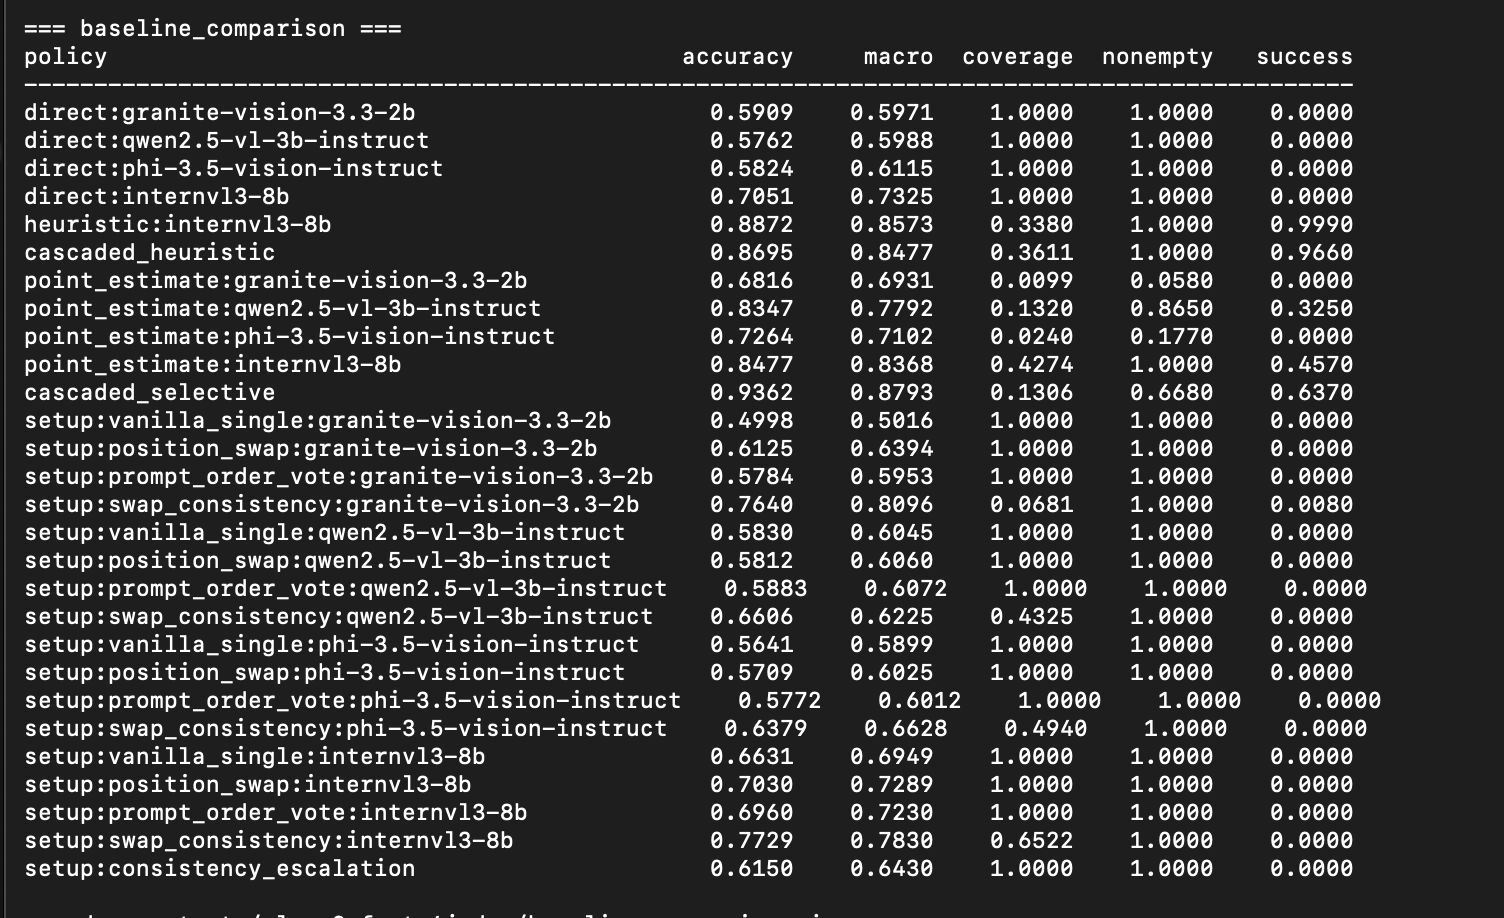
\includegraphics[width=\textwidth]{baseline_comparison.jpeg}
    \caption{Terminal output of the baseline comparison over 1,000 repeated
    group-safe calibration--test splits. Accuracy is calculated conditionally
    on answered examples, while coverage, nonempty rate, and target success
    are averaged across repetitions.}
    \label{fig:baseline-comparison-output}
\end{figure*}

\begin{figure*}[t]
    \centering
    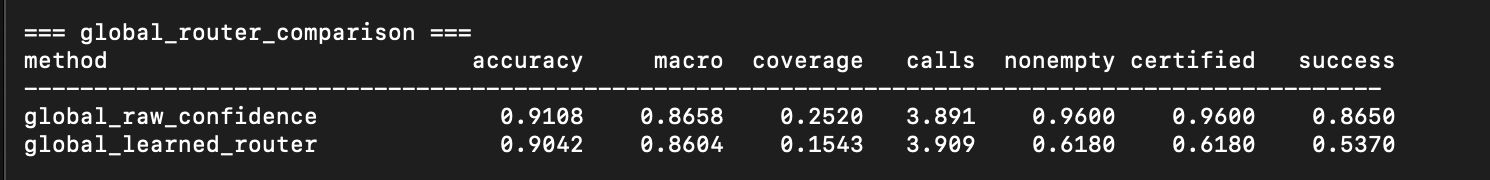
\includegraphics[width=\textwidth]{endtoend.jpeg}
    \caption{Terminal output of the end-to-end routing comparison. The global
    raw-confidence and learned-router policies are evaluated on the same 1,000
    repeated router-training, certification, and test partitions.}
    \label{fig:endtoend-output}
\end{figure*}

Figures~\ref{fig:baseline-comparison-output}
and~\ref{fig:endtoend-output} shows the terminal outputs produced by the
cached-policy evaluation.

% Upload screenshots to an Overleaf folder such as figures/ and uncomment
% the figure environments below after confirming the filenames.
%
% \begin{figure}[H]
%   \centering
%   \includegraphics[width=0.92\linewidth]{figures/dataset_preparation.png}
%   \caption{Dataset preparation and validation from an actual run.}
%   \label{fig:dataset-run}
% \end{figure}
%
% \begin{figure}[H]
%   \centering
%   \includegraphics[width=0.92\linewidth]{figures/baseline_evaluation.png}
%   \caption{Baseline evaluation using the documented configuration.}
%   \label{fig:baseline-run}
% \end{figure}
%
% \begin{figure}[H]
%   \centering
%   \includegraphics[width=0.92\linewidth]{figures/global_router_evaluation.png}
%   \caption{End-to-end router evaluation and saved metrics.}
%   \label{fig:router-run}
% \end{figure}

% =========================================================
\section{Results and Findings}

\begin{table*}[t]
\centering
\footnotesize
\setlength{\tabcolsep}{6pt}
\begin{tabular}{@{}lrrrrr@{}}
\toprule
\textbf{Policy} & \textbf{Acc.} & \textbf{Macro} & \textbf{Cov.} & \textbf{Nonempty} & \textbf{Success} \\
\midrule
\method{direct:granite-vision-3.3-2b} & .5909 & .5971 & 1.0000 & 1.0000 & .0000 \\
\method{direct:qwen2.5-vl-3b-instruct} & .5762 & .5988 & 1.0000 & 1.0000 & .0000 \\
\method{direct:phi-3.5-vision-instruct} & .5824 & .6115 & 1.0000 & 1.0000 & .0000 \\
\method{direct:internvl3-8b} & .7051 & .7325 & 1.0000 & 1.0000 & .0000 \\
\rowcolor{pale}\method{heuristic:internvl3-8b} & .8872 & .8573 & .3380 & 1.0000 & .9990 \\
\rowcolor{pale}\method{cascaded_heuristic} & .8695 & .8477 & .3611 & 1.0000 & .9660 \\
\method{point_estimate:granite-vision-3.3-2b} & .6816 & .6931 & .0099 & .0580 & .0000 \\
\method{point_estimate:qwen2.5-vl-3b-instruct} & .8347 & .7792 & .1320 & .8650 & .3250 \\
\method{point_estimate:phi-3.5-vision-instruct} & .7264 & .7102 & .0240 & .1770 & .0000 \\
\method{point_estimate:internvl3-8b} & .8477 & .8368 & .4274 & 1.0000 & .4570 \\
\rowcolor{pale}\method{cascaded_selective} & .9362 & .8793 & .1306 & .6680 & .6370 \\
\midrule
\method{setup:vanilla_single:granite-vision-3.3-2b} & .4998 & .5016 & 1.0000 & 1.0000 & .0000 \\
\method{setup:position_swap:granite-vision-3.3-2b} & .6125 & .6394 & 1.0000 & 1.0000 & .0000 \\
\method{setup:prompt_order_vote:granite-vision-3.3-2b} & .5784 & .5953 & 1.0000 & 1.0000 & .0000 \\
\method{setup:swap_consistency:granite-vision-3.3-2b} & .7640 & .8096 & .0681 & 1.0000 & .0080 \\
\method{setup:vanilla_single:qwen2.5-vl-3b-instruct} & .5830 & .6045 & 1.0000 & 1.0000 & .0000 \\
\method{setup:position_swap:qwen2.5-vl-3b-instruct} & .5812 & .6060 & 1.0000 & 1.0000 & .0000 \\
\method{setup:prompt_order_vote:qwen2.5-vl-3b-instruct} & .5883 & .6072 & 1.0000 & 1.0000 & .0000 \\

\method{setup:swap_consistency:qwen2.5-vl-3b-instruct} & .6606 & .6225 & .4325 & 1.0000 & .0000 \\
\method{setup:vanilla_single:phi-3.5-vision-instruct} & .5641 & .5899 & 1.0000 & 1.0000 & .0000 \\
\method{setup:position_swap:phi-3.5-vision-instruct} & .5709 & .6025 & 1.0000 & 1.0000 & .0000 \\
\method{setup:prompt_order_vote:phi-3.5-vision-instruct} & .5772 & .6012 & 1.0000 & 1.0000 & .0000 \\
\method{setup:swap_consistency:phi-3.5-vision-instruct} & .6379 & .6628 & .4940 & 1.0000 & .0000 \\
\method{setup:vanilla_single:internvl3-8b} & .6631 & .6949 & 1.0000 & 1.0000 & .0000 \\
\method{setup:position_swap:internvl3-8b} & .7030 & .7289 & 1.0000 & 1.0000 & .0000 \\
\method{setup:prompt_order_vote:internvl3-8b} & .6960 & .7230 & 1.0000 & 1.0000 & .0000 \\
\method{setup:swap_consistency:internvl3-8b} & .7729 & .7830 & .6522 & 1.0000 & .0000 \\
\method{setup:consistency_escalation} & .6150 & .6430 & 1.0000 & 1.0000 & .0000 \\
\bottomrule
\end{tabular}
\caption{Baseline Results}
\label{tab:baseline-results}
\end{table*}

\subsection{Baseline Results}
% Abhinav
All the baseline results are summarized in Table \ref{tab:baseline-results}. We notice that basically most of the baselines do not meet our required threshold that we set ($1 - \alpha = 0.85$). Only 3 of them (heuristic, cascade with heursitic, cascaded selective evaluation, these are highlighted in the table too) meet this standard. Out of these three,the highest accuracy is for the cascaded selective evaluation method itself (but this should not matter that much as long as accuracy is above the threshold) - the concerning part here is that the coverage is only 13 \%.  The other two methods - although have lower accuracy (but still above the threshold) - have higher coverage - sitting around 33-35\%. This suggests that we can somehow improve the cascaded selective method to increase coverage even if that takes a small hit in accuracy, as long as its above the $1- \alpha$ bound set by us.

% All baseline results are summarized in Table~\ref{tab:baseline-results}. Most baselines do not meet the target selective accuracy of $1-\alpha=0.85$. Only three methods meet this target: the single-judge heuristic, the heuristic cascade, and cascaded selective evaluation. Cascaded selective evaluation achieves the highest selective accuracy at 93.62\%, but its coverage is only 13.06\%. In comparison, the single-judge heuristic and heuristic cascade achieve lower selective accuracies of 88.72\% and 86.95\%, respectively, but substantially higher coverages of 33.80\% and 36.11\%. These results show that the certified cascade is overly conservative: it exceeds the accuracy target by a large margin while abstaining on most examples. This motivates modifying the certification procedure to improve coverage while maintaining selective accuracy above the required $85\%$ threshold.

\subsection{End-to-End Routing Results}
The four-judge end-to-end experiment uses 1,000 repeated splits. Each split contains approximately 200 router-training examples, 300 certification examples, and 500 test examples. The two end-to-end policies use identical partitions within each repetition.

\begin{table}[t]
\centering
\small
\resizebox{\linewidth}{!}{%
\begin{tabular}{lrrrrrrr}
\toprule
\textbf{Method} & \textbf{Accuracy} & \textbf{Macro acc.} & \textbf{Coverage} & \textbf{Mean calls} & \textbf{Nonempty} & \textbf{Certified} & \textbf{Target success} \\
\midrule
Global raw confidence & 91.08\% & 86.58\% & 25.20\% & 3.891 & 96.00\% & 96.00\% & 86.50\% \\
Global learned router & 90.42\% & 86.04\% & 15.43\% & 3.909 & 61.80\% & 61.80\% & 53.70\% \\
\bottomrule
\end{tabular}%
}
% \caption{End-to-end routing results reported in the README. Accuracy is conditional on answering; target success is a per-repetition empirical quantity.}
\caption{End-to-end routing results. Accuracy is conditional on answering; target success is a per-repetition empirical quantity.}
\label{tab:global-results}
\end{table}

On this benchmark, global raw-confidence certification has higher reported coverage than the learned-router policy while retaining selective accuracy above 90\%. Compared with the stage-wise certified baseline, raw-confidence end-to-end certification increases reported coverage from 13.06\% to 25.20\%, a difference of 12.14 percentage points. The average number of judges called is 3.891, so the coverage gain does not demonstrate a substantial reduction in judge computation.

% The learned router is a negative result for this sample size: it certifies fewer repetitions and provides lower coverage than raw confidence. The repository notes suggest that fitting a multi-feature correctness model from approximately 200 router-training examples may have introduced variance. The observed comparison is consistent with that explanation, but does not by itself establish the cause.
The learned router is a negative result at this sample size: it certifies fewer repetitions and provides lower coverage than raw confidence. The explanation is that approximately 200 router-training examples are insufficient to reliably fit the multi-feature correctness model, leading to greater estimation variance. The observed results are consistent with this explanation, but do not establish it as the cause.

\subsection{Interpreting Certification and Target Success}
For the global raw-confidence policy, the reported certificate is found in 96.0\% of repetitions and the policy meets the test target in 86.5\% of all repetitions. Among repetitions with a certificate, target success is $86.5/96.0\approx90.1\%$, close to the nominal 90\% confidence level in this benchmark. This is an empirical repeated-split check; it does not replace the mathematical assumptions underlying the certificate.

% The original baseline comparison and the end-to-end comparison do not use the same test partition sizes: the original comparison allocates about 300 examples to calibration and 700 to testing, while the end-to-end method reserves training, certification and test partitions of roughly 200, 300 and 500 examples. Therefore, the headline comparison with the stage-wise policy should be described as a comparison of repeated-split aggregates, not a paired estimate on identical test examples.
The original baseline and end-to-end comparisons use different partition sizes. The baseline comparison allocates approximately 300 examples to calibration and 700 to testing, whereas the end-to-end comparison allocates approximately 200 examples to router training, 300 to certification, and 500 to testing. Consequently, the reported results compare aggregate performance across repeated splits rather than paired performance on identical test examples.

% =========================================================
\section{Discussion and Limitations}
Our evaluation highlights a clear trade-off between reliability and coverage. None of the four individual VLM judges reaches the target 85\% accuracy when forced to answer every sample, with direct accuracies between 57.62\% and 70.51\%. End-2-end certification with raw confidence successfully guarantees selective accuracy (91.08\%) while nearly doubling coverage from 13.06\% to 25.20\%. However, this coverage gain does not significantly cut computation, as the cascade queries an average of 3.89 out of 4 judges per answered query before reaching sufficient confidence.

The experiments also find surprising failure cases and results. Training a complex 11-feature learned router on only $\sim$200 examples led to overfitting and high variance, certifying far fewer splits (61.8\%) and yielding lower coverage (15.43\%) than raw confidence. Further, the judges exhibited severe positional and prompt sensitivity: models frequently flipped their preferences simply when candidate response order was swapped or when longer responses were presented. While filtering for response-order consistency raised accuracy, it caused drop in coverage.

Several limitations apply to these conclusions. All findings are derived from a 1,000-example benchmark of four specific open-weight VLMs with pre-cached inferences, meaning repeated splits test sensitivity to partition choices rather than independent datasets. In addition, dataset peculiarities such as length bias and differing label annotations (e.g., human corrections in RLHF-V versus pairwise preference votes in VisionArena) affect model agreement. These trade offs and routing behaviors may differ on other multimodal distributions, different judge sequences, or larger proprietary models.

% =========================================================
\section{Conclusion}
The project extends cascaded selective evaluation from text-only judges to a multimodal preference setting using four open-weight VLM judge families. The current repository implements established baseline policies and compares stage-wise certification with end-to-end certification of a frozen policy. In the reported 1,000-example benchmark, raw-confidence end-to-end certification obtains 91.08\% selective accuracy at 25.20\% coverage, compared with 93.62\% accuracy at 13.06\% coverage for the stage-wise certified cascade. The learned router does not improve the trade-off in this experiment. These results motivate further testing of routing-score design and coverage under group-safe repeated splits; conclusions should remain restricted to the current benchmark and reported configuration.

% =========================================================
\section{Team Contributions for Assignment 2}

Every member took part in the discussion and ideation meetings, while giving all relevant inputs based on their experiences. Experiments and report writing was mutually divided, each member reviewed everyone's work and gave feedbacks.

\begin{table}[H]
\centering
\small
\begin{tabularx}{\linewidth}{p{0.29\linewidth} p{0.14\linewidth} Y}
\toprule
\textbf{Member} & \textbf{Score (\%)} & \textbf{Actual Assignment 2 contribution} \\
\midrule
Parth Dembla & 12.5 & Documented mentor feedback, results, and provided ideation inputs. \\
Ridham Patel Vijaykumar & 12.5 & Proposed novel method, executed cluster runs, and fixed issues. \\
Anurag Singh & 12.5 & Built code harness and experiment structure for VLM evaluation. \\
Arjun B. Dikshit & 12.5 & Prepared dataset processing pipeline according to TA feedback. \\
Abhinav Khot & 12.5 & Analyzed and documented the baseline policies and cascades. \\
Shardul Junagade & 12.5 & Documented feedback and results, and contributed conceptual ideas. \\
Shriniket Behera & 12.5 & Documented feedback, analyzed findings, and provided ideation inputs. \\
Rathod Yuvraj Rajubhai & 12.5 & Built code harness and experiment execution framework. \\
\midrule
\textbf{Total} & \textbf{100} & \\
\bottomrule
\end{tabularx}
\caption{Actual group contributions to Assignment 2.}
\label{tab:contributions}
\end{table}

% =========================================================
\bibliographystyle{acl_natbib}
\bibliography{custom}

\end{document}
